
%(BEGIN_QUESTION)
% Copyright 2015, Tony R. Kuphaldt, released under the Creative Commons Attribution License (v 1.0)
% This means you may do almost anything with this work of mine, so long as you give me proper credit

A Koyo CLICK PLC controls the start-up of a gas-fuel furnace, using an {\it event drum} instruction.  The purpose of this sequence is to safely ``purge'' the furnace of any residual fuel gas vapors using fresh air before attempting to ignite it:

\begin{itemize}
\item{} {\bf Inputs} 
\item{} {\tt X001} -- ``Purge start'' pushbutton (momentary NO)
\item{} {\tt X002} -- ``Ignition start'' pushbutton (momentary NO)
\item{} {\tt X003} -- ``Shutdown'' pushbutton (momentary NO)
\item{} {\tt X004} -- Flame sensor -- {\it PLC input energizes when flame detected}
\end{itemize}

\begin{itemize}
\item{} {\bf Outputs} 
\item{} {\tt Y001} -- Combustion air valve -- {\it energizing this PLC output opens the air valve to the furnace}
\item{} {\tt Y002} -- Fuel gas valve -- {\it energizing this PLC output opens the fuel gas valve to the furnace}
\item{} {\tt Y003} -- ``Purge complete'' lamp
\item{} {\tt Y004} -- Spark ignition coil
\end{itemize}

\filbreak

\begin{itemize}
\item{} {\bf Step description} 
\item{} Step 1 -- Waiting to purge
\item{} Step 2 -- Purging combustion chamber
\item{} Step 3 -- Chamber purged, waiting to start
\item{} Step 4 -- Furnace running
\end{itemize}

$$\includegraphics[width=15.5cm]{i00458x01.eps}$$

\filbreak

$$\includegraphics[width=15.5cm]{i00458x02.eps}$$

Analyze this furnace control program, and then explain what each instruction does (including the practical function of each timer instruction).  Also, identify all conditions that will shut down this system (returning the drum to step 1).

\vskip 20pt \vbox{\hrule \hbox{\strut \vrule{} {\bf Suggestions for Socratic discussion} \vrule} \hrule}

\begin{itemize}
\item{} Why is a {\it purge time} so important to the safe operation of a gas fuel furnace?
\item{} Explain the purpose of the NO contact instruction addressed to the bit {\tt \_Always\_ON} ({\tt SC1}).
\item{} Suppose you were helping another technician troubleshoot a burner problem in this furnace, and in the process of doing so had to start up and shut down the furnace several times.  The technician you are working with gets impatient and tells you to edit the PLC program so that he won't have to wait so long for the furnace to re-purge itself every start-up cycle.  Which portion of the program controls the purge time?  Would you do what the other technician tells you to do?  Why or why not?
\item{} Suppose the programmer writing this program forgot to include the normally-open Y002 contact in the rung leading to the drum instruction's {\it reset} input.  How would this omission affect the program's operation?
\item{} Suppose the programmer writing this program forgot to include the normally-closed Y004 contact in the rung leading to the drum instruction's {\it reset} input.  How would this omission affect the program's operation?
\end{itemize}

\underbar{file i00458}
%(END_QUESTION)





%(BEGIN_ANSWER)


%(END_ANSWER)





%(BEGIN_NOTES)

Timer T1 controls the purge cycle (480 seconds = 8 minutes).

\vskip 10pt

Timer T2 controls the ``wait'' time, allowing time between purge completion and burner start.  The drum will reset to step 1 if no one has pushed the ``Ignition start'' button within 5 minutes of purge completion.

\vskip 10pt

Timer T3 controls the ignition time delay (10 seconds), giving that much time for the burner to light.  If there is no proof of flame within this amount of time, the drum will reset to step 1.

\vskip 10pt

Finally, someone pressing the ``Shutdown'' button will reset the drum to setp 1.

%INDEX% PLC, ladder logic program analysis and explanation (Koyo CLICK)
%INDEX% Process: furnace safety purge controller 

%(END_NOTES)


